\section{Risultati e Discussione}

In questa sezione vengono analizzati i risultati ottenuti, confrontando un approccio preliminare basato su una GAN incondizionata con il sistema C-DCWGAN-GP finale.

\subsection{Analisi Preliminare: Il problema della scarsità di dati}

Inizialmente, è stato condotto un esperimento per testare la capacità di  apprendere la distribuzione della sola classe minoritaria, utilizzando esclusivamente i 1341 campioni reali disponibili. 
I risultati sono stati insoddisfacenti: la rete non è stata in grado di convergere verso una rappresentazione realistica, producendo immagini affette da artefatti evidenti e segnali di mode collapse. L'integrazione di questi campioni nel dataset di addestramento ha portato a un degrado delle performance della ResNet18. Questo fallimento conferma un'ipotesi critica: una GAN necessita di una massa critica di dati per mappare correttamente le feature spaziali. Limitando il training alle sole immagini sane, il modello non ha beneficiato del confronto con le caratteristiche morfologiche della polmonite, fallendo nel definire i confini della classe.

\begin{figure}[ht]
    \centering
    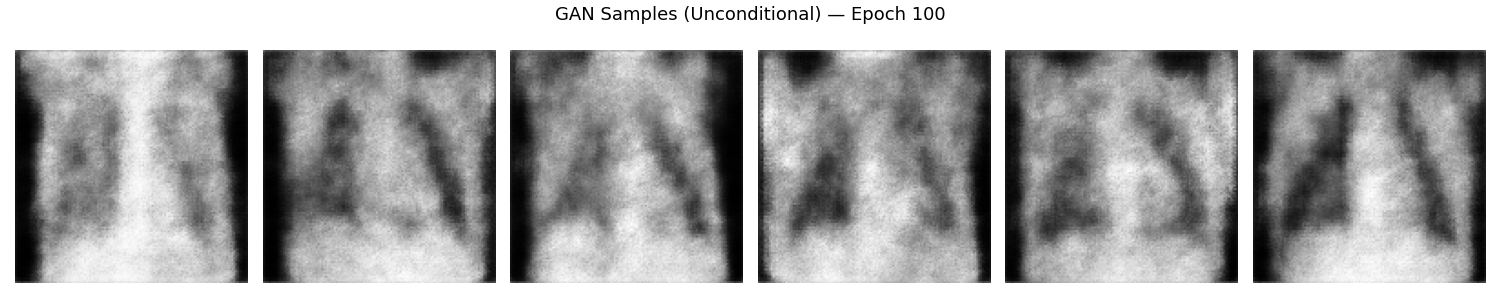
\includegraphics[width=\columnwidth]{images/samples_epoch_100_uncond.png} 
    \caption{Evoluzione dei campioni generati per il modello incondizionato.}
    \label{fig:samples_unconditional}
\end{figure}

\subsection{Risultati Finali: Data Augmentation tramite C-DCWGAN-GP}

L'adozione della Conditional GAN, addestrata sull'intero pool di dati, ha ribaltato i risultati. Sfruttando le informazioni provenienti da entrambe le classi, il generatore ha prodotto campioni sintetici di alta qualità che hanno permesso un bilanciamento efficace del dataset.

\paragraph{Analisi Quantitativa}
Il confronto tra la Baseline (Phase 1) e il modello addestrato con i dati sintetici (Phase 3) evidenzia un netto miglioramento in tutte le metriche chiave \ref{fig:cm1}, \ref{tab:confronto_classi}.

\begin{figure}[ht]
    \centering
    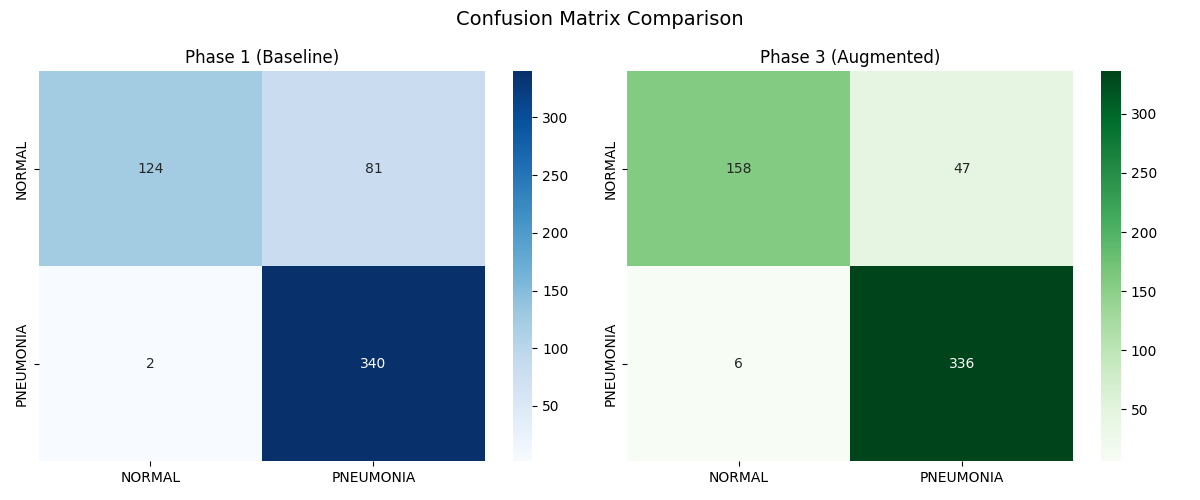
\includegraphics[width=\columnwidth]{images/cm_comparison-4.png} 
    \caption{Confronto tra matrici di confusioni baseline vs augmented.}
    \label{fig:cm1}
\end{figure}

\begin{table}[h]
\centering
\resizebox{\columnwidth}{!}{%
    \begin{tabular}{l|cc|cc}
    \toprule
    & \multicolumn{2}{c|}{\textbf{Normal}} & \multicolumn{2}{c}{\textbf{Pneumonia}} \\ 
    \textbf{Modello} & Rec. & F1 & Prec. & F1 \\ \midrule
    Baseline & 0.60 & 0.74 & 0.80 & 0.89 \\
    \textbf{Augm.} & \textbf{0.77} & \textbf{0.85} & \textbf{0.87} & \textbf{0.92} \\ \midrule
    \textit{Delta} & +16\% & +11\% & +7\% & +3\% \\ \bottomrule
    \end{tabular}%
}
\caption{Confronto prestazioni per classe: Baseline vs Augmented (Phase 3). Si osserva il significativo recupero di Recall nella classe minoritaria.}
\label{tab:confronto_classi}
\end{table}

\begin{figure*}[t]
    \centering
    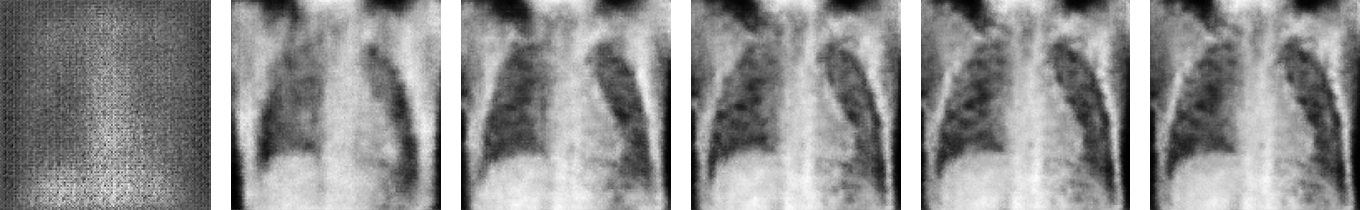
\includegraphics[width=\textwidth]{images/progressione_gan.png} 
    \caption{Progressione dell'addestramento della C-DCWGAN-GP: campioni generati ogni 20 epoche. Si osserva il passaggio dal rumore iniziale alla definizione dei dettagli anatomici polmonari.}
    \label{fig:progressione_completa}
\end{figure*}

Il dato più significativo è l'incremento del Recall per la classe NORMAL (da 0.60 a 0.77). Questo indica che il modello originale tendeva a classificare erroneamente molti pazienti sani come malati (falsi positivi), a causa della scarsa rappresentazione dei polmoni sani nel training set. L'introduzione di dati sintetici ha permesso alla ResNet18 di imparare a distinguere con molta più precisione le sottili differenze visive, portando l'accuratezza globale oltre il 90%.

\subsection{Analisi Qualitativa e Training Stability}

L'analisi dei log di Weights  Biases (WandB) ha confermato la stabilità della C-DCWGAN-GP. A differenza dell'esperimento 1, la Wasserstein Loss ha mostrato una decrescita regolare, correlata visivamente a un progressivo miglioramento dei campioni generati.

I sample generati \ref{fig:progressione_completa} mostrano una corretta ricostruzione delle strutture costali e dei campi polmonari, confermando che il condizionamento della label e l'aumento dei dati di training totali hanno permesso al modello di superare i limiti della scarsità di dati iniziale.

